\documentclass[11pt]{article}\usepackage[]{graphicx}\usepackage[]{color}
%% maxwidth is the original width if it is less than linewidth
%% otherwise use linewidth (to make sure the graphics do not exceed the margin)
\makeatletter
\def\maxwidth{ %
  \ifdim\Gin@nat@width>\linewidth
    \linewidth
  \else
    \Gin@nat@width
  \fi
}
\makeatother

\definecolor{fgcolor}{rgb}{0.345, 0.345, 0.345}
\newcommand{\hlnum}[1]{\textcolor[rgb]{0.686,0.059,0.569}{#1}}%
\newcommand{\hlstr}[1]{\textcolor[rgb]{0.192,0.494,0.8}{#1}}%
\newcommand{\hlcom}[1]{\textcolor[rgb]{0.678,0.584,0.686}{\textit{#1}}}%
\newcommand{\hlopt}[1]{\textcolor[rgb]{0,0,0}{#1}}%
\newcommand{\hlstd}[1]{\textcolor[rgb]{0.345,0.345,0.345}{#1}}%
\newcommand{\hlkwa}[1]{\textcolor[rgb]{0.161,0.373,0.58}{\textbf{#1}}}%
\newcommand{\hlkwb}[1]{\textcolor[rgb]{0.69,0.353,0.396}{#1}}%
\newcommand{\hlkwc}[1]{\textcolor[rgb]{0.333,0.667,0.333}{#1}}%
\newcommand{\hlkwd}[1]{\textcolor[rgb]{0.737,0.353,0.396}{\textbf{#1}}}%

\usepackage{framed}
\makeatletter
\newenvironment{kframe}{%
 \def\at@end@of@kframe{}%
 \ifinner\ifhmode%
  \def\at@end@of@kframe{\end{minipage}}%
  \begin{minipage}{\columnwidth}%
 \fi\fi%
 \def\FrameCommand##1{\hskip\@totalleftmargin \hskip-\fboxsep
 \colorbox{shadecolor}{##1}\hskip-\fboxsep
     % There is no \\@totalrightmargin, so:
     \hskip-\linewidth \hskip-\@totalleftmargin \hskip\columnwidth}%
 \MakeFramed {\advance\hsize-\width
   \@totalleftmargin\z@ \linewidth\hsize
   \@setminipage}}%
 {\par\unskip\endMakeFramed%
 \at@end@of@kframe}
\makeatother

\definecolor{shadecolor}{rgb}{.97, .97, .97}
\definecolor{messagecolor}{rgb}{0, 0, 0}
\definecolor{warningcolor}{rgb}{1, 0, 1}
\definecolor{errorcolor}{rgb}{1, 0, 0}
\newenvironment{knitrout}{}{} % an empty environment to be redefined in TeX

\usepackage{alltt}
\usepackage{amsmath}
\usepackage{listings}
\usepackage{stmaryrd}
\usepackage{bbm}
\usepackage{amsmath}
\usepackage{mathtools}
\usepackage{pdfpages}
\usepackage{breqn}



\newcount\colveccount
\newcommand*\colvec[1]{
        \global\colveccount#1
        \begin{pmatrix}
        \colvecnext
}
\def\colvecnext#1{
        #1
        \global\advance\colveccount-1
        \ifnum\colveccount>0
                \\
                \expandafter\colvecnext
        \else
                \end{pmatrix}
        \fi
}
\newcommand{\argmin}{\arg\!\min}

\author{Thibault Doutre, Student ID 26980469}
\title{STAT230 HW 7 \\
University of California, Berkeley}
\date{\today}
\IfFileExists{upquote.sty}{\usepackage{upquote}}{}
\begin{document}

\maketitle
\section{Lab 11}
\begin{knitrout}
\definecolor{shadecolor}{rgb}{0.969, 0.969, 0.969}\color{fgcolor}\begin{kframe}
\begin{alltt}
\hlcom{# Compute log likelihood}
\hlstd{log_likelihood_aux} \hlkwb{=} \hlkwa{function}\hlstd{(}\hlkwc{theta}\hlstd{,}\hlkwc{X}\hlstd{)\{}
  \hlstd{n} \hlkwb{=} \hlkwd{lengthgth}\hlstd{(X)}
  \hlstd{n}\hlopt{*}\hlkwd{log}\hlstd{(theta)} \hlopt{-} \hlnum{2}\hlopt{*}\hlkwd{sum}\hlstd{(}\hlkwd{log}\hlstd{(theta}\hlopt{+}\hlstd{X))}
\hlstd{\}}
\hlstd{log_likelihood} \hlkwb{=} \hlkwd{Vectorize}\hlstd{(log_likelihood_aux)}

\hlcom{# Change variable theta<-exp(phi)}
\hlstd{log_likelihood_phi_aux} \hlkwb{=} \hlkwa{function}\hlstd{(}\hlkwc{phi}\hlstd{,}\hlkwc{X}\hlstd{)\{}
  \hlstd{n} \hlkwb{=} \hlkwd{length}\hlstd{(X)}
  \hlstd{n}\hlopt{*}\hlstd{phi} \hlopt{-} \hlnum{2}\hlopt{*}\hlkwd{sum}\hlstd{(}\hlkwd{log}\hlstd{(}\hlkwd{exp}\hlstd{(phi)}\hlopt{+}\hlstd{X))}
\hlstd{\}}

\hlstd{MLE} \hlkwb{=} \hlkwa{function} \hlstd{(}\hlkwc{X}\hlstd{)\{}
  \hlstd{f} \hlkwb{=} \hlkwa{function}\hlstd{(}\hlkwc{phi}\hlstd{)\{}\hlopt{-}\hlkwd{log_likelihood_phi_aux}\hlstd{(phi,X)\}}
  \hlstd{opt} \hlkwb{=} \hlkwd{optim}\hlstd{(}\hlnum{0}\hlstd{,f,}
              \hlkwc{method}\hlstd{=}\hlstr{"Brent"}\hlstd{,}
              \hlkwc{lower} \hlstd{=} \hlnum{0}\hlstd{,}
              \hlkwc{upper} \hlstd{=} \hlnum{10}\hlstd{)}
  \hlstd{theta_hat} \hlkwb{=} \hlkwd{exp}\hlstd{(opt}\hlopt{$}\hlstd{par)}
  \hlstd{theta_hat}
\hlstd{\}}
\end{alltt}
\end{kframe}
\end{knitrout}
\subsection{Generate uniform RV}
\begin{knitrout}
\definecolor{shadecolor}{rgb}{0.969, 0.969, 0.969}\color{fgcolor}\begin{kframe}
\begin{alltt}
\hlkwd{set.seed}\hlstd{(}\hlnum{1}\hlstd{)}
\hlstd{theta_hat_values} \hlkwb{=} \hlkwd{c}\hlstd{()}
\hlkwa{for} \hlstd{(i} \hlkwa{in} \hlnum{1}\hlopt{:}\hlnum{1000}\hlstd{)\{}
  \hlcom{# Generate data}
  \hlstd{U} \hlkwb{=} \hlkwd{runif}\hlstd{(}\hlnum{50}\hlstd{)}
  \hlstd{theta} \hlkwb{=} \hlnum{25}
  \hlstd{X} \hlkwb{=} \hlstd{theta}\hlopt{*}\hlkwd{sapply}\hlstd{(U,}\hlkwa{function}\hlstd{(}\hlkwc{x}\hlstd{) x}\hlopt{/}\hlstd{(}\hlnum{1}\hlopt{-}\hlstd{x))}
  \hlcom{# Compute MLE}
  \hlstd{theta_hat} \hlkwb{=} \hlkwd{MLE}\hlstd{(X)}
  \hlstd{theta_hat_values} \hlkwb{=} \hlkwd{c}\hlstd{(theta_hat_values,theta_hat)}
\hlstd{\}}
\end{alltt}
\end{kframe}
\end{knitrout}
\subsection{Plot histogram}
\begin{knitrout}
\definecolor{shadecolor}{rgb}{0.969, 0.969, 0.969}\color{fgcolor}\begin{kframe}
\begin{alltt}
\hlkwd{hist}\hlstd{(theta_hat_values,}
     \hlkwc{xlab} \hlstd{=} \hlstr{"theta_hat"}\hlstd{,}
     \hlkwc{main} \hlstd{=} \hlstr{"Realizations of MLE"}\hlstd{)}
\end{alltt}
\end{kframe}
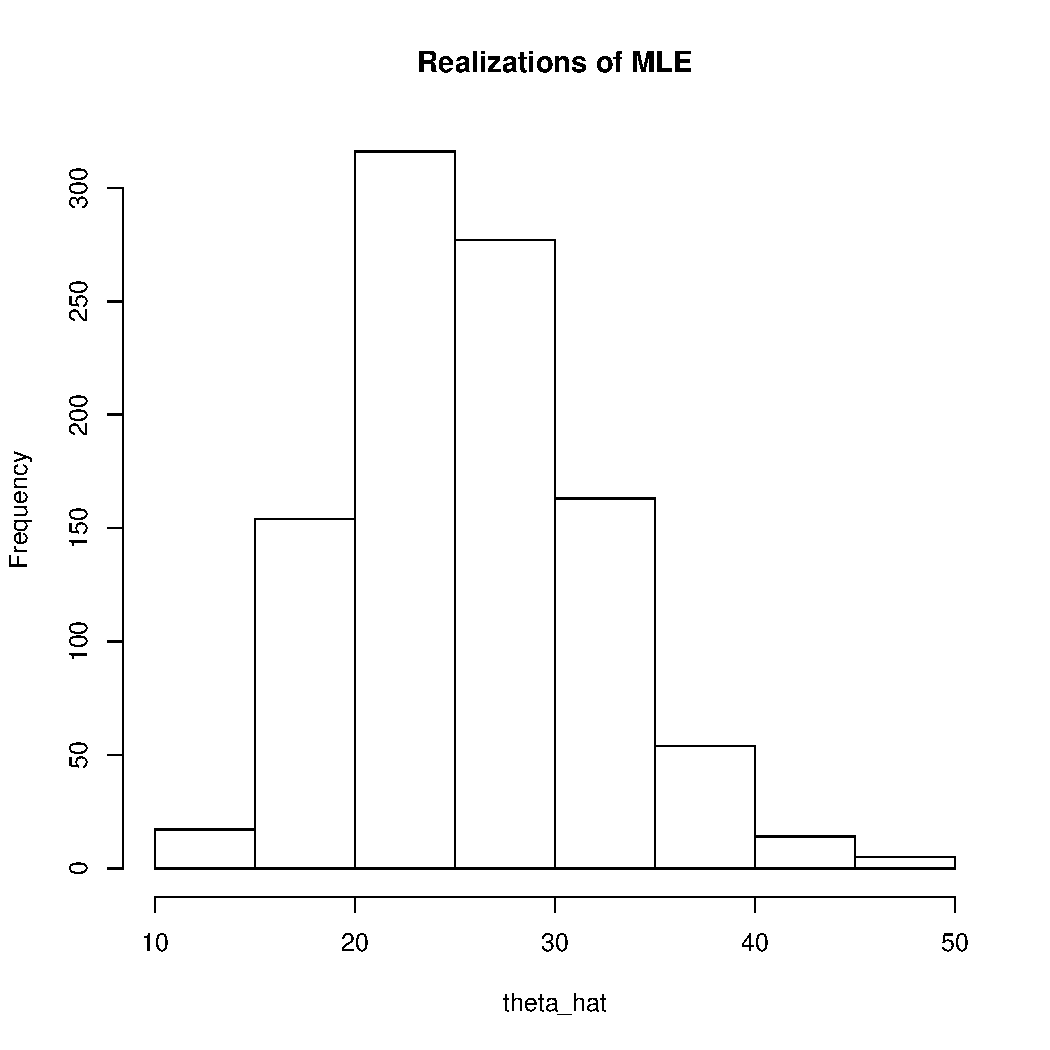
\includegraphics[width=\maxwidth]{figure/unnamed-chunk-4-1} 

\end{knitrout}
\subsection{Mean/SD}
\begin{knitrout}
\definecolor{shadecolor}{rgb}{0.969, 0.969, 0.969}\color{fgcolor}\begin{kframe}
\begin{alltt}
\hlstd{mu} \hlkwb{=} \hlkwd{mean}\hlstd{(theta_hat_values)}
\hlstd{mu}
\end{alltt}
\begin{lstlisting}[basicstyle=\ttfamily,breaklines=true]
## [1] 25.72292
\end{lstlisting}
\begin{alltt}
\hlstd{sigma} \hlkwb{=} \hlkwd{sd}\hlstd{(theta_hat_values)}
\hlstd{sigma}
\end{alltt}
\begin{lstlisting}[basicstyle=\ttfamily,breaklines=true]
## [1] 6.04452
\end{lstlisting}
\begin{alltt}
\hlstd{fisher_info} \hlkwb{=} \hlkwa{function}\hlstd{(}\hlkwc{theta}\hlstd{)\{}
  \hlnum{1}\hlopt{/}\hlstd{(}\hlnum{3}\hlopt{*}\hlstd{theta}\hlopt{^}\hlnum{2}\hlstd{)}
\hlstd{\}}
\hlcom{# Comparison}
\hlstd{asympt_var} \hlkwb{=} \hlnum{1}\hlopt{/}\hlkwd{sqrt}\hlstd{(}\hlnum{50}\hlopt{*}\hlkwd{fisher_info}\hlstd{(}\hlnum{25}\hlstd{))}
\hlstd{sigma}
\end{alltt}
\begin{lstlisting}[basicstyle=\ttfamily,breaklines=true]
## [1] 6.04452
\end{lstlisting}
\begin{alltt}
\hlstd{asympt_var}\hlopt{-}\hlstd{sigma}
\end{alltt}
\begin{lstlisting}[basicstyle=\ttfamily,breaklines=true]
## [1] 0.07920436
\end{lstlisting}
\end{kframe}
\end{knitrout}
The asymptotic sd is equal to $1/\sqrt{50I_{\theta}(25)}$. Therefore they shoud be equal for an infinite number of simulations, c.f. formula Example 4, Chapter 7.

\subsection{Bonus}
6.\\ 
The asymptotic sd should be more accurate to estimate SE because it is a limit of the sd of a n-sized sample. \\
\noindent
7.\\
The asymptotic sd doubles and the fisher info is divided by 4, see formula. The standard deviation of the observed info will also double and will still tend to the asymptotic sd as n grows to infinity.

\section{Lab 12}

\begin{knitrout}
\definecolor{shadecolor}{rgb}{0.969, 0.969, 0.969}\color{fgcolor}\begin{kframe}
\begin{alltt}
\hlstd{data} \hlkwb{=} \hlkwd{read.table}\hlstd{(}\hlstr{"pac01.dat"}\hlstd{)}
\hlkwd{head}\hlstd{(data)}
\end{alltt}
\begin{lstlisting}[basicstyle=\ttfamily,breaklines=true]
##   V1 V2 V3 V4 V5 V6 V7 V8 V9 V10 V11 V12 V13 V14 V15 V16
## 1 23  1  4  8  4  2  3 37  1   2   2  40   0   1  22   9
## 2 45  1  1  8  1  1  3 39  6   0   1  -1   1   0   0   0
## 3 39  2  3  8  1  1  3 40  1   3   2  46   0   0  18   2
## 4 16  1  3  8  7  0  3 35  4   8  11  -1   6   1  24  15
## 5 53  2  1  8  5  0  1 41  1   1   2  54   0   0  17   2
## 6 42  1  1  8  7  0  1 42  1   1   2  50   0   0  10   1
##     V17   V18 V19 V20  V21 V22 V23 V24    V25    V26 V27
## 1 15002 15002   1   0  445   1   1   0 216162 330502  91
## 2  2200 28300   1   0 1451   1   1   2 259495 324334  91
## 3 26100 28300   1   0 1451   1   2   1 205681 324334  91
## 4     0 28300   1   0 1451   1   3   0 218787 356936  91
## 5 23000 23000   1   0 4356   1   1   0 200660 347911  91
## 6 44297 44297   1   0 4357   1   1   0 206279 351372  91
\end{lstlisting}
\begin{alltt}
\hlkwd{names}\hlstd{(data)}\hlkwb{=}\hlkwd{c}\hlstd{(}\hlstr{"AGE"}\hlstd{,}
              \hlstr{"SEX"}\hlstd{,}
              \hlstr{"RACE"}\hlstd{,}
              \hlstr{"ETHNICITY"}\hlstd{,}
              \hlstr{"MARITAL"}\hlstd{,}
              \hlstr{"NUMKIDS"}\hlstd{,}
              \hlstr{"FAMPERS"}\hlstd{,}
              \hlstr{"EDLEVEL"}\hlstd{,}
              \hlstr{"LABSTAT"}\hlstd{,}
              \hlstr{"CLASSWORK"}\hlstd{,}
              \hlstr{"FULLPART"}\hlstd{,}
              \hlstr{"HOURS"}\hlstd{,}
              \hlstr{"WHYNOTWORK"}\hlstd{,}
              \hlstr{"INSCHOOL"}\hlstd{,}
              \hlstr{"INDUSTRY"}\hlstd{,}
              \hlstr{"OCCUPATION"}\hlstd{,}
              \hlstr{"PINCOME"}\hlstd{,}
              \hlstr{"INCFAM"}\hlstd{,}
              \hlstr{"CITIZEN"}\hlstd{,}
              \hlstr{"IMMIGYR"}\hlstd{,}
              \hlstr{"HHSEQNUM"}\hlstd{,}
              \hlstr{"FSEQNUM"}\hlstd{,}
              \hlstr{"PERSCODE"}\hlstd{,}
              \hlstr{"SPOUCODE"}\hlstd{,}
              \hlstr{"FINALWGT"}\hlstd{,}
              \hlstr{"MARCHWGT"}\hlstd{,}
              \hlstr{"STATE"}\hlstd{)}

\hlkwd{head}\hlstd{(data)}
\end{alltt}
\begin{lstlisting}[basicstyle=\ttfamily,breaklines=true]
##   AGE SEX RACE ETHNICITY MARITAL NUMKIDS FAMPERS EDLEVEL
## 1  23   1    4         8       4       2       3      37
## 2  45   1    1         8       1       1       3      39
## 3  39   2    3         8       1       1       3      40
## 4  16   1    3         8       7       0       3      35
## 5  53   2    1         8       5       0       1      41
## 6  42   1    1         8       7       0       1      42
##   LABSTAT CLASSWORK FULLPART HOURS WHYNOTWORK INSCHOOL
## 1       1         2        2    40          0        1
## 2       6         0        1    -1          1        0
## 3       1         3        2    46          0        0
## 4       4         8       11    -1          6        1
## 5       1         1        2    54          0        0
## 6       1         1        2    50          0        0
##   INDUSTRY OCCUPATION PINCOME INCFAM CITIZEN IMMIGYR
## 1       22          9   15002  15002       1       0
## 2        0          0    2200  28300       1       0
## 3       18          2   26100  28300       1       0
## 4       24         15       0  28300       1       0
## 5       17          2   23000  23000       1       0
## 6       10          1   44297  44297       1       0
##   HHSEQNUM FSEQNUM PERSCODE SPOUCODE FINALWGT MARCHWGT
## 1      445       1        1        0   216162   330502
## 2     1451       1        1        2   259495   324334
## 3     1451       1        2        1   205681   324334
## 4     1451       1        3        0   218787   356936
## 5     4356       1        1        0   200660   347911
## 6     4357       1        1        0   206279   351372
##   STATE
## 1    91
## 2    91
## 3    91
## 4    91
## 5    91
## 6    91
\end{lstlisting}
\begin{alltt}
\hlstd{subset} \hlkwb{=} \hlstd{data[,}\hlkwd{c}\hlstd{(}\hlstr{"LABSTAT"}\hlstd{,}\hlstr{"AGE"}\hlstd{,}\hlstr{"SEX"}\hlstd{,}\hlstr{"RACE"}\hlstd{,}\hlstr{"EDLEVEL"}\hlstd{)]}
\hlkwd{head}\hlstd{(subset)}
\end{alltt}
\begin{lstlisting}[basicstyle=\ttfamily,breaklines=true]
##   LABSTAT AGE SEX RACE EDLEVEL
## 1       1  23   1    4      37
## 2       6  45   1    1      39
## 3       1  39   2    3      40
## 4       4  16   1    3      35
## 5       1  53   2    1      41
## 6       1  42   1    1      42
\end{lstlisting}
\end{kframe}
\end{knitrout}

\subsection{}
I chose to only define binary random variables in order to avoid putting more weight on some factors. The baseline individual in the model, choose a person who is male, non- white, age 16–19, and did not graduate from high school. It corresponds to zero values variables in the model.
\begin{knitrout}
\definecolor{shadecolor}{rgb}{0.969, 0.969, 0.969}\color{fgcolor}\begin{kframe}
\begin{alltt}
\hlcom{# Split age}
\hlstd{split_age1} \hlkwb{=} \hlkwd{rep}\hlstd{(}\hlnum{0}\hlstd{,}\hlkwd{length}\hlstd{(data}\hlopt{$}\hlstd{AGE))}
\hlstd{split_age2} \hlkwb{=} \hlkwd{rep}\hlstd{(}\hlnum{0}\hlstd{,}\hlkwd{length}\hlstd{(data}\hlopt{$}\hlstd{AGE))}
\hlstd{split_age3} \hlkwb{=} \hlkwd{rep}\hlstd{(}\hlnum{0}\hlstd{,}\hlkwd{length}\hlstd{(data}\hlopt{$}\hlstd{AGE))}

\hlstd{split_age1[data}\hlopt{$}\hlstd{AGE}\hlopt{>=}\hlnum{20} \hlopt{&} \hlstd{data}\hlopt{$}\hlstd{AGE}\hlopt{<=}\hlnum{39}\hlstd{]} \hlkwb{=} \hlnum{1}\hlcom{#"20–39"}
\hlstd{split_age2[data}\hlopt{$}\hlstd{AGE}\hlopt{>=}\hlnum{40} \hlopt{&} \hlstd{data}\hlopt{$}\hlstd{AGE}\hlopt{<=}\hlnum{64}\hlstd{]} \hlkwb{=} \hlnum{1}\hlcom{#"40-64"}
\hlstd{split_age3[data}\hlopt{$}\hlstd{AGE}\hlopt{>=}\hlnum{65}\hlstd{]} \hlkwb{=} \hlnum{1}\hlcom{#"65+"}

\hlcom{# Split Race}
\hlstd{split_race} \hlkwb{=} \hlkwd{rep}\hlstd{(}\hlnum{0}\hlstd{,}\hlkwd{length}\hlstd{(data}\hlopt{$}\hlstd{RACE))}
\hlstd{split_race[data}\hlopt{$}\hlstd{RACE}\hlopt{!=}\hlnum{1}\hlstd{]} \hlkwb{=} \hlnum{1}\hlcom{#"white"}

\hlcom{# Split Education level}
\hlstd{split_edlevel1} \hlkwb{=} \hlkwd{rep}\hlstd{(}\hlnum{0}\hlstd{,}\hlkwd{length}\hlstd{(data}\hlopt{$}\hlstd{EDLEVEL))}
\hlstd{split_edlevel2} \hlkwb{=} \hlkwd{rep}\hlstd{(}\hlnum{0}\hlstd{,}\hlkwd{length}\hlstd{(data}\hlopt{$}\hlstd{EDLEVEL))}
\hlstd{split_edlevel1[data}\hlopt{$}\hlstd{EDLEVEL}\hlopt{==}\hlnum{39}\hlstd{]} \hlkwb{=} \hlnum{1}\hlcom{#"HS "}
\hlstd{split_edlevel2[data}\hlopt{$}\hlstd{EDLEVEL}\hlopt{>=}\hlnum{40}\hlstd{]} \hlkwb{=} \hlnum{1}\hlcom{#"HS+"}

\hlcom{# Split SEX}
\hlstd{split_sex} \hlkwb{=} \hlkwd{rep}\hlstd{(}\hlnum{NA}\hlstd{,}\hlkwd{length}\hlstd{(data}\hlopt{$}\hlstd{SEX))}
\hlstd{split_sex[data}\hlopt{$}\hlstd{SEX}\hlopt{==}\hlnum{1}\hlstd{]}\hlkwb{=}\hlnum{0}\hlcom{#"M"}
\hlstd{split_sex[data}\hlopt{$}\hlstd{SEX}\hlopt{==}\hlnum{2}\hlstd{]}\hlkwb{=}\hlnum{1}\hlcom{#"F"}

\hlstd{features} \hlkwb{=} \hlkwd{data.frame}\hlstd{(}\hlkwc{LABSTAT} \hlstd{=} \hlkwd{as.numeric}\hlstd{(data}\hlopt{$}\hlstd{LABSTAT}\hlopt{==}\hlnum{1}\hlstd{),}
                      \hlkwc{SEX} \hlstd{=} \hlkwd{as.numeric}\hlstd{(split_sex),}
                      \hlkwc{AGE1} \hlstd{=} \hlkwd{as.numeric}\hlstd{(split_age1),}
                      \hlkwc{AGE2} \hlstd{=} \hlkwd{as.numeric}\hlstd{(split_age2),}
                      \hlkwc{AGE3} \hlstd{=} \hlkwd{as.numeric}\hlstd{(split_age3),}
                      \hlkwc{RACE} \hlstd{=} \hlkwd{as.numeric}\hlstd{(split_race),}
                      \hlkwc{EDLEVEL1} \hlstd{=} \hlkwd{as.numeric}\hlstd{(split_edlevel1),}
                      \hlkwc{EDLEVEL2} \hlstd{=} \hlkwd{as.numeric}\hlstd{(split_edlevel2))}
\hlkwd{head}\hlstd{(features)}
\end{alltt}
\begin{lstlisting}[basicstyle=\ttfamily,breaklines=true]
##   LABSTAT SEX AGE1 AGE2 AGE3 RACE EDLEVEL1 EDLEVEL2
## 1       1   0    1    0    0    1        0        0
## 2       0   0    0    1    0    0        1        0
## 3       1   1    1    0    0    1        0        1
## 4       0   0    0    0    0    1        0        0
## 5       1   1    0    1    0    0        0        1
## 6       1   0    0    1    0    0        0        1
\end{lstlisting}
\begin{alltt}
\hlkwd{any}\hlstd{(}\hlkwd{is.na}\hlstd{(features))}
\end{alltt}
\begin{lstlisting}[basicstyle=\ttfamily,breaklines=true]
## [1] FALSE
\end{lstlisting}
\begin{alltt}
\hlcom{## # 1. }
\hlstd{design} \hlkwb{=} \hlstd{features[,}\hlopt{-}\hlnum{1}\hlstd{]}
\hlstd{design}\hlopt{$}\hlstd{Intercept} \hlkwb{=} \hlkwd{as.numeric}\hlstd{(}\hlnum{1}\hlstd{)}
\hlkwd{head}\hlstd{(design)}
\end{alltt}
\begin{lstlisting}[basicstyle=\ttfamily,breaklines=true]
##   SEX AGE1 AGE2 AGE3 RACE EDLEVEL1 EDLEVEL2 Intercept
## 1   0    1    0    0    1        0        0         1
## 2   0    0    1    0    0        1        0         1
## 3   1    1    0    0    1        0        1         1
## 4   0    0    0    0    1        0        0         1
## 5   1    0    1    0    0        0        1         1
## 6   0    0    1    0    0        0        1         1
\end{lstlisting}
\begin{alltt}
\hlstd{names_features} \hlkwb{=} \hlkwd{names}\hlstd{(design)}
\hlstd{design} \hlkwb{=} \hlkwd{as.matrix}\hlstd{(design)}


\hlcom{# Size of design matrix}
\hlkwd{dim}\hlstd{(design)}
\end{alltt}
\begin{lstlisting}[basicstyle=\ttfamily,breaklines=true]
## [1] 13803     8
\end{lstlisting}
\begin{alltt}
\hlstd{Y}\hlkwb{=}\hlstd{features[,}\hlnum{1}\hlstd{]}
\end{alltt}
\end{kframe}
\end{knitrout}
\subsection{}
I use pracma library in order to find the maximum likelihood estimator.
\begin{knitrout}
\definecolor{shadecolor}{rgb}{0.969, 0.969, 0.969}\color{fgcolor}\begin{kframe}
\begin{alltt}
\hlkwd{library}\hlstd{(pracma)}

\hlstd{Eta} \hlkwb{=} \hlkwa{function}\hlstd{(}\hlkwc{x}\hlstd{)\{}
  \hlkwd{sapply}\hlstd{(x,}\hlkwa{function}\hlstd{(}\hlkwc{x}\hlstd{)} \hlnum{1}\hlopt{/}\hlstd{(}\hlnum{1}\hlopt{+}\hlkwd{exp}\hlstd{(}\hlopt{-}\hlstd{x)))}
\hlstd{\}}

\hlcom{# Negative log likelihood}
\hlstd{loss} \hlkwb{=} \hlkwa{function}\hlstd{(}\hlkwc{beta}\hlstd{)\{}
  \hlstd{x} \hlkwb{=} \hlstd{design} \hlopt \hlstd{beta}
  \hlopt{-}\hlstd{(}\hlkwd{sum}\hlstd{(Y}\hlopt{*}\hlkwd{log}\hlstd{(}\hlkwd{Eta}\hlstd{(x))}\hlopt{+}\hlstd{(}\hlnum{1}\hlopt{-}\hlstd{Y)}\hlopt{*}\hlkwd{log}\hlstd{(}\hlnum{1}\hlopt{-}\hlkwd{Eta}\hlstd{(x))))}
\hlstd{\}}

\hlstd{beta0} \hlkwb{=} \hlkwd{as.matrix}\hlstd{(}\hlkwd{rep}\hlstd{(}\hlnum{0}\hlstd{,}\hlkwd{dim}\hlstd{(design)[}\hlnum{2}\hlstd{]))}
\hlkwd{loss}\hlstd{(beta0)}
\end{alltt}
\begin{lstlisting}[basicstyle=\ttfamily,breaklines=true]
## [1] 9567.511
\end{lstlisting}
\begin{alltt}
\hlstd{mini} \hlkwb{=} \hlkwd{fminsearch}\hlstd{(loss,beta0)}
\hlstd{beta_hat} \hlkwb{=} \hlstd{mini}\hlopt{$}\hlstd{xval}
\hlkwd{names}\hlstd{(beta_hat)} \hlkwb{<-} \hlstd{names_features}
\hlstd{beta_hat}
\end{alltt}
\begin{lstlisting}[basicstyle=\ttfamily,breaklines=true]
##        SEX       AGE1       AGE2       AGE3       RACE 
## -0.7176359  1.3289470  1.2365739 -1.6667350 -0.1826282 
##   EDLEVEL1   EDLEVEL2  Intercept 
##  0.7369803  0.9931386 -0.5787865
\end{lstlisting}
\end{kframe}
\end{knitrout}
We can also fit the logit with the glm function directly:
\begin{knitrout}
\definecolor{shadecolor}{rgb}{0.969, 0.969, 0.969}\color{fgcolor}\begin{kframe}
\begin{alltt}
\hlcom{## Alternative}
\hlstd{glm.fit} \hlkwb{<-} \hlkwd{glm}\hlstd{(LABSTAT} \hlopt{~}\hlstd{. ,} \hlkwc{data} \hlstd{= features,} \hlkwc{family} \hlstd{=} \hlstr{"binomial"}\hlstd{)}
\hlkwd{summary}\hlstd{(glm.fit)}
\end{alltt}
\begin{lstlisting}[basicstyle=\ttfamily,breaklines=true]
## 
## Call:
## glm(formula = LABSTAT ~ ., family = "binomial", data = features)
## 
## Deviance Residuals: 
##     Min       1Q   Median       3Q      Max  
## -1.9517  -0.8754   0.5925   0.8144   2.5251  
## 
## Coefficients:
##             Estimate Std. Error z value Pr(>|z|)    
## (Intercept) -0.57880    0.06953  -8.324  < 2e-16 ***
## SEX         -0.71753    0.04088 -17.551  < 2e-16 ***
## AGE1         1.32888    0.07487  17.750  < 2e-16 ***
## AGE2         1.23652    0.07563  16.350  < 2e-16 ***
## AGE3        -1.66690    0.10143 -16.434  < 2e-16 ***
## RACE        -0.18265    0.05034  -3.628 0.000285 ***
## EDLEVEL1     0.73705    0.05657  13.029  < 2e-16 ***
## EDLEVEL2     0.99318    0.05067  19.601  < 2e-16 ***
## ---
## Signif. codes:  
## 0 '***' 0.001 '**' 0.01 '*' 0.05 '.' 0.1 ' ' 1
## 
## (Dispersion parameter for binomial family taken to be 1)
## 
##     Null deviance: 18319  on 13802  degrees of freedom
## Residual deviance: 14879  on 13795  degrees of freedom
## AIC: 14895
## 
## Number of Fisher Scoring iterations: 4
\end{lstlisting}
\end{kframe}
\end{knitrout}

\subsection{}
\begin{knitrout}
\definecolor{shadecolor}{rgb}{0.969, 0.969, 0.969}\color{fgcolor}\begin{kframe}
\begin{alltt}
\hlcom{# Standard errors}
\hlkwd{summary}\hlstd{(glm.fit)}\hlopt{$}\hlstd{coefficients[,}\hlnum{2}\hlstd{]}
\end{alltt}
\begin{lstlisting}[basicstyle=\ttfamily,breaklines=true]
## (Intercept)         SEX        AGE1        AGE2        AGE3 
##  0.06953246  0.04088345  0.07486672  0.07562729  0.10143142 
##        RACE    EDLEVEL1    EDLEVEL2 
##  0.05034075  0.05657165  0.05066913
\end{lstlisting}
\end{kframe}
\end{knitrout}

\subsection{}
When looking at the sign of the coefficients we can first say that employment is positively correlated with having been to high school or above, since the baseline is no high school and the coefficients for EDLEVEL1 and EDLEVEL2 are positive. Similarly, we can also conclude that beign either a woman or non-white has a bad impact 
on employment.
Moreover, it is important to notice that the p-values are all very small, which shows the importance of all the features used to predict the outcome.

\subsection{}

First of all there is no way to correctly quantify the education, so we cannot use a real valued variable and perform regression. As a matter of fact we have categorical variables. We use dummy variables in order to avoid giving more weight to some variables: the way of assigning factors matters in the regression in the sense that the linear model gives more importance to categories with a bigger factor.
\subsection{}
The fact that most of women give birth may impact their employment since the employers know that they might not be able to work for a while.
Moreover, the SEX variable might be correlated with the edication level for example. It is known that women have less access to education that men for some reasons and it might impact their employment.
LABSTAT codes more than 4 are relevant because women aremore likely not to work than men do. Therefore they might not be looking for a job, which is generally not the case for men.


\end{document}









